\chapter{Experimental testing}
\label{chp:5}

\graphicspath{{chapter_5_Experimentaltesting/figures}}

\section{Introduction}
To gain a better insight on the mechanical properties of FFF produced ABS parts and the bulk filament, a series of experimental tensile tests were conducted. These tests are used afterwards as validation for the constitutive (elastic and non-elastic models) to predict the mechanical behaviour. First a set of tensile tests in the three principle direction were conducted according to ISO 527\cite{De2013NEN-EN-ISO527-4}\cite{Afd2016NEN-EN-ISO527-2}. Since FFF produced parts show significant anisotropy and have no accepted testing standard, the results were non-satisfactory. Due to the geometry of the dogbone shape incorporated by the ISO 527 standard, premature failure occured. Therefore an additional test was conducted using the ASTM D 3039 \cite{ASTM2008Standard3039} standard, which defines a different geometrical shape, generally used for long fibre composites. Additionally, a ASTM D 3039 test with wall layers in the XY direction and a set of YX[45]n samples has been tested for shear. Finally, a set of filament tested to determine the bulk properties. These properties are important to implement in the RVE model, since it will determine how the plastic response of the bulk material will be. 

\section{Methods and procedures}
In this section the methods and procedures of the experiments will be presented. All samples were produced and tested with the same hardware and parameters (with some exceptions). The tests were performed with the corresponding ISO 527 and ASTM D 3039 standards.
The samples were produced on a UMS5 machine with Ultimaker black ABS\cite{Ultimaker2018TechnicalABS}, a road width of 0.4 and a speed of 35mm/min. For each set five samples were tested in the 3 principle directions (YX[0] XY[0] ZX[0] of figure \ref{fig:coordinates}). The samples were tested on a Zwick/Roell 10kN universal testing machine. The test was strain driven and included an extensometer of 50 mm gauge length that immediately processes the stress strain data in the Test Expert software. Before testing the samples, the dimensions of the cross section were measured. It should be noted that the true dimension of the cross section can vary significantly from the nominal production dimensions. Additionally, the roughness of the sample makes it more difficult to exactly determine the cross section of the sample. This results in a inaccuracy of the true measured values for stress and Young's moduli. 

The strain rates differ slightly per testing standard (ISO 527 and ASTM D 3039). Both advise a strain rate of approximately 1\%/min for the calculation of the E modulus (both standards  calculate the E modulus between 0.05\% and 0.25\% strain).  ISO 527 specifies a speed of 1mm/min while ASTM D 3039 specifies a test speed of 2mm/min for the calculation of the E modulus, both correspond to approximately 1\%/min, since both samples are in the range of 100-200 mm.

After the determination of the E modulus, which is calculated by a linear regression calculation between 0.05\% strain and 0.25\% strain, the strain rate can be adjusted. Since thermoplastics show significant viscoelastic behaviour this can significantly alter the obtained stress-strain curve. Both standards give a wide range of possible testing speeds, ISO 527 ranges from 0.125 to 500 mm/min. ASTM 3039 specifies that failure should occur in between 1 and 10 minutes after starting the tensile test. The tests conducted in literature often remained on the same strain rate as was defined for the E modulus. To make a better comparison between the tests from the different standards a strain rate of 2mm/min was chosen for the strain rate after the calculation of the E modulus.
In the plastic region, the yield point is defined as the top of the slope were the derivative of the stress strain curve is zero. If this point is not reached (due to failure), the yield point is defined as at the same point as the break point.

\subsection{ISO 527}
The ISO 527-2 standard \cite{Afd2016NEN-EN-ISO527-2} prescribes a tensile test standard for thermoplastics. The 1A sample \ref{fig:ISO527} was used to perform this test. The thickness of the sample is 4 mm.
\begin{figure}[H]
    \centering
    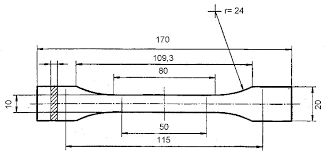
\includegraphics[width=0.50\textwidth]{chapter_5_Experimentaltesting/figures/ISO527specimen.png}
    \caption{Dimensions of the ISO 527 dogbone used}
    \label{fig:ISO527}
\end{figure}
\subsection{ASTM D 3039}
The ASTM D 3039 standard \cite{Afd2016NEN-EN-ISO527-2} prescribes a tensile test standard for long fibre composites. This standard has been used by Rodriguez \cite{Rodriguez2001MechanicalInvestigation} to prevent  stress concentrations occurring at the fillets of the ISO 527 specimens. The geometry of the ASTM sample used was a simple rectangle with a nominal dimension of 110 x 20 x 4 mm, including an image is otiose. The ASTM standard advised to use a form of tabs at the interface of the grips and specimen to minimize the damage and stress concentration. The tabs should be slightly longer than the area where the grips are clamped. The tabs used for the ASTM 3039 sample were 20 x 30mm and made out of thick (approximatly 1mm) paper.

\subsection{Ultimaker ABS Filament}
To determine the bulk properties of the Ultimaker ABS Filament a set of single filament pieces were tested. There is currently no testing standard for testing thick (nominal diameter of 2.85mm) thermoplastic filament. For the process parameters the settings of ISO 527 specified by the Ultimaker Technical Datatsheet \cite{Ultimaker2018TechnicalABS} were largely followed. These include the E modulus testing of 1 mm/min followed by a strain rate of 50 mm/min. The hardware used is similar to the setup for the FFF produced samples. Ideally, special grips for filament would be used, since these were not available regular grips were used. 
FFF filament is inherently bent, to solve this problem the filament was straighten out and clamped before a pre-load of 5 MPa was induced to align the filament. 

\section{Results}
The results are presented in stress strain curves with the corresponding testing standard, images of the tested samples are presented were relevant. Every set includes a minimum of 5 tested samples. Since averaging the curves is nearly impossible, the longest or most representative response is plotted and additionally the yield points of the set are added. This gives a representation of the yielding behaviour and its consistency. 

\subsection{ISO 527}
In figure \ref{fig:ISO527results} and table \label{tab:ISO527results} the results are presented of the ISO 527 samples with two wall layers.
\begin{figure}[H]
    \centering
    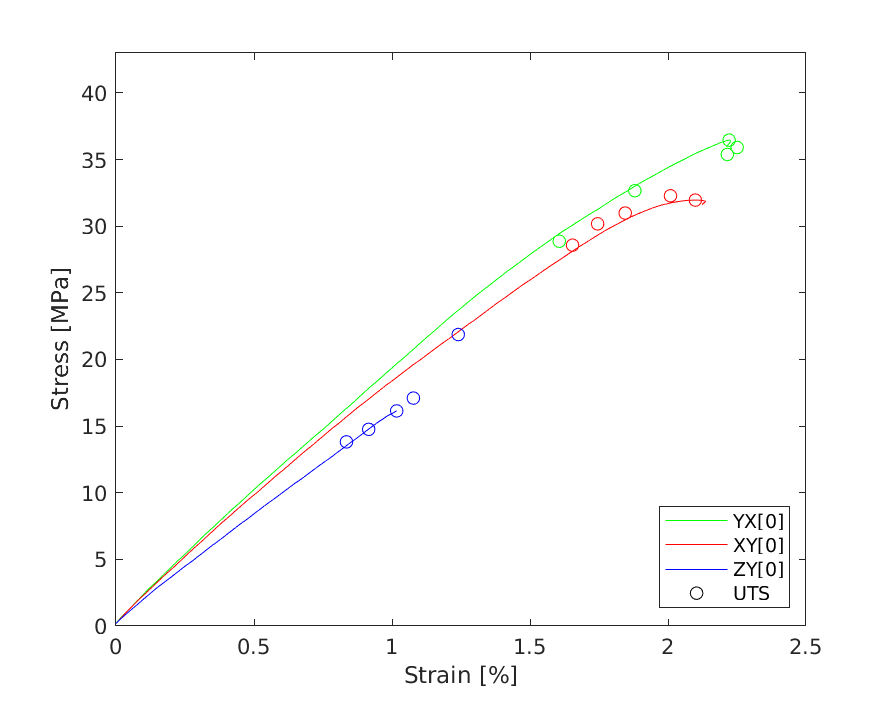
\includegraphics[width=0.80\textwidth]{chapter_5_Experimentaltesting/figures/ISOTensiletests.png}
    \caption{Stress strain curves of the ISO 527 samples}
    \label{fig:ISO527results}
\end{figure}

\begin{table}[ht]
\centering
\caption{Properties of the ISO 527 tests in the 3 principle directions}
          \label{tab:ISO527results}
\begin{tabular}{ p{1.5cm}p{1cm}p{1cm}p{1cm}p{1cm}p{1cm}p{1cm}  }
\hline
direction & $E$ avg. [MPa] & $E$ std. dev. & $\sigma_y$avg. [MPa] & $\sigma_y$ std. dev. & $\epsilon_y$ avg. [\%] & $\epsilon_y$   std. dev. \\
 \hline
1 (YX[0]) & 2019 & 53 & 33.8 & 4.5 & 1.84 & 0.37 \\
2 (XY[0]) & 1974 & 77 & 30.8 & 1.3 & 1.87 & 0.16 \\
3 (ZY[0]) & 1793 & 119 & 16.3 & 2.8 & 0.95 & 0.19\\
 \hline
\end{tabular}
\end{table}



In figure \ref{fig:ISO527specimen} the tested specimen of the ISO 527 samples are shown. 
\begin{figure}[H]
    \centering
    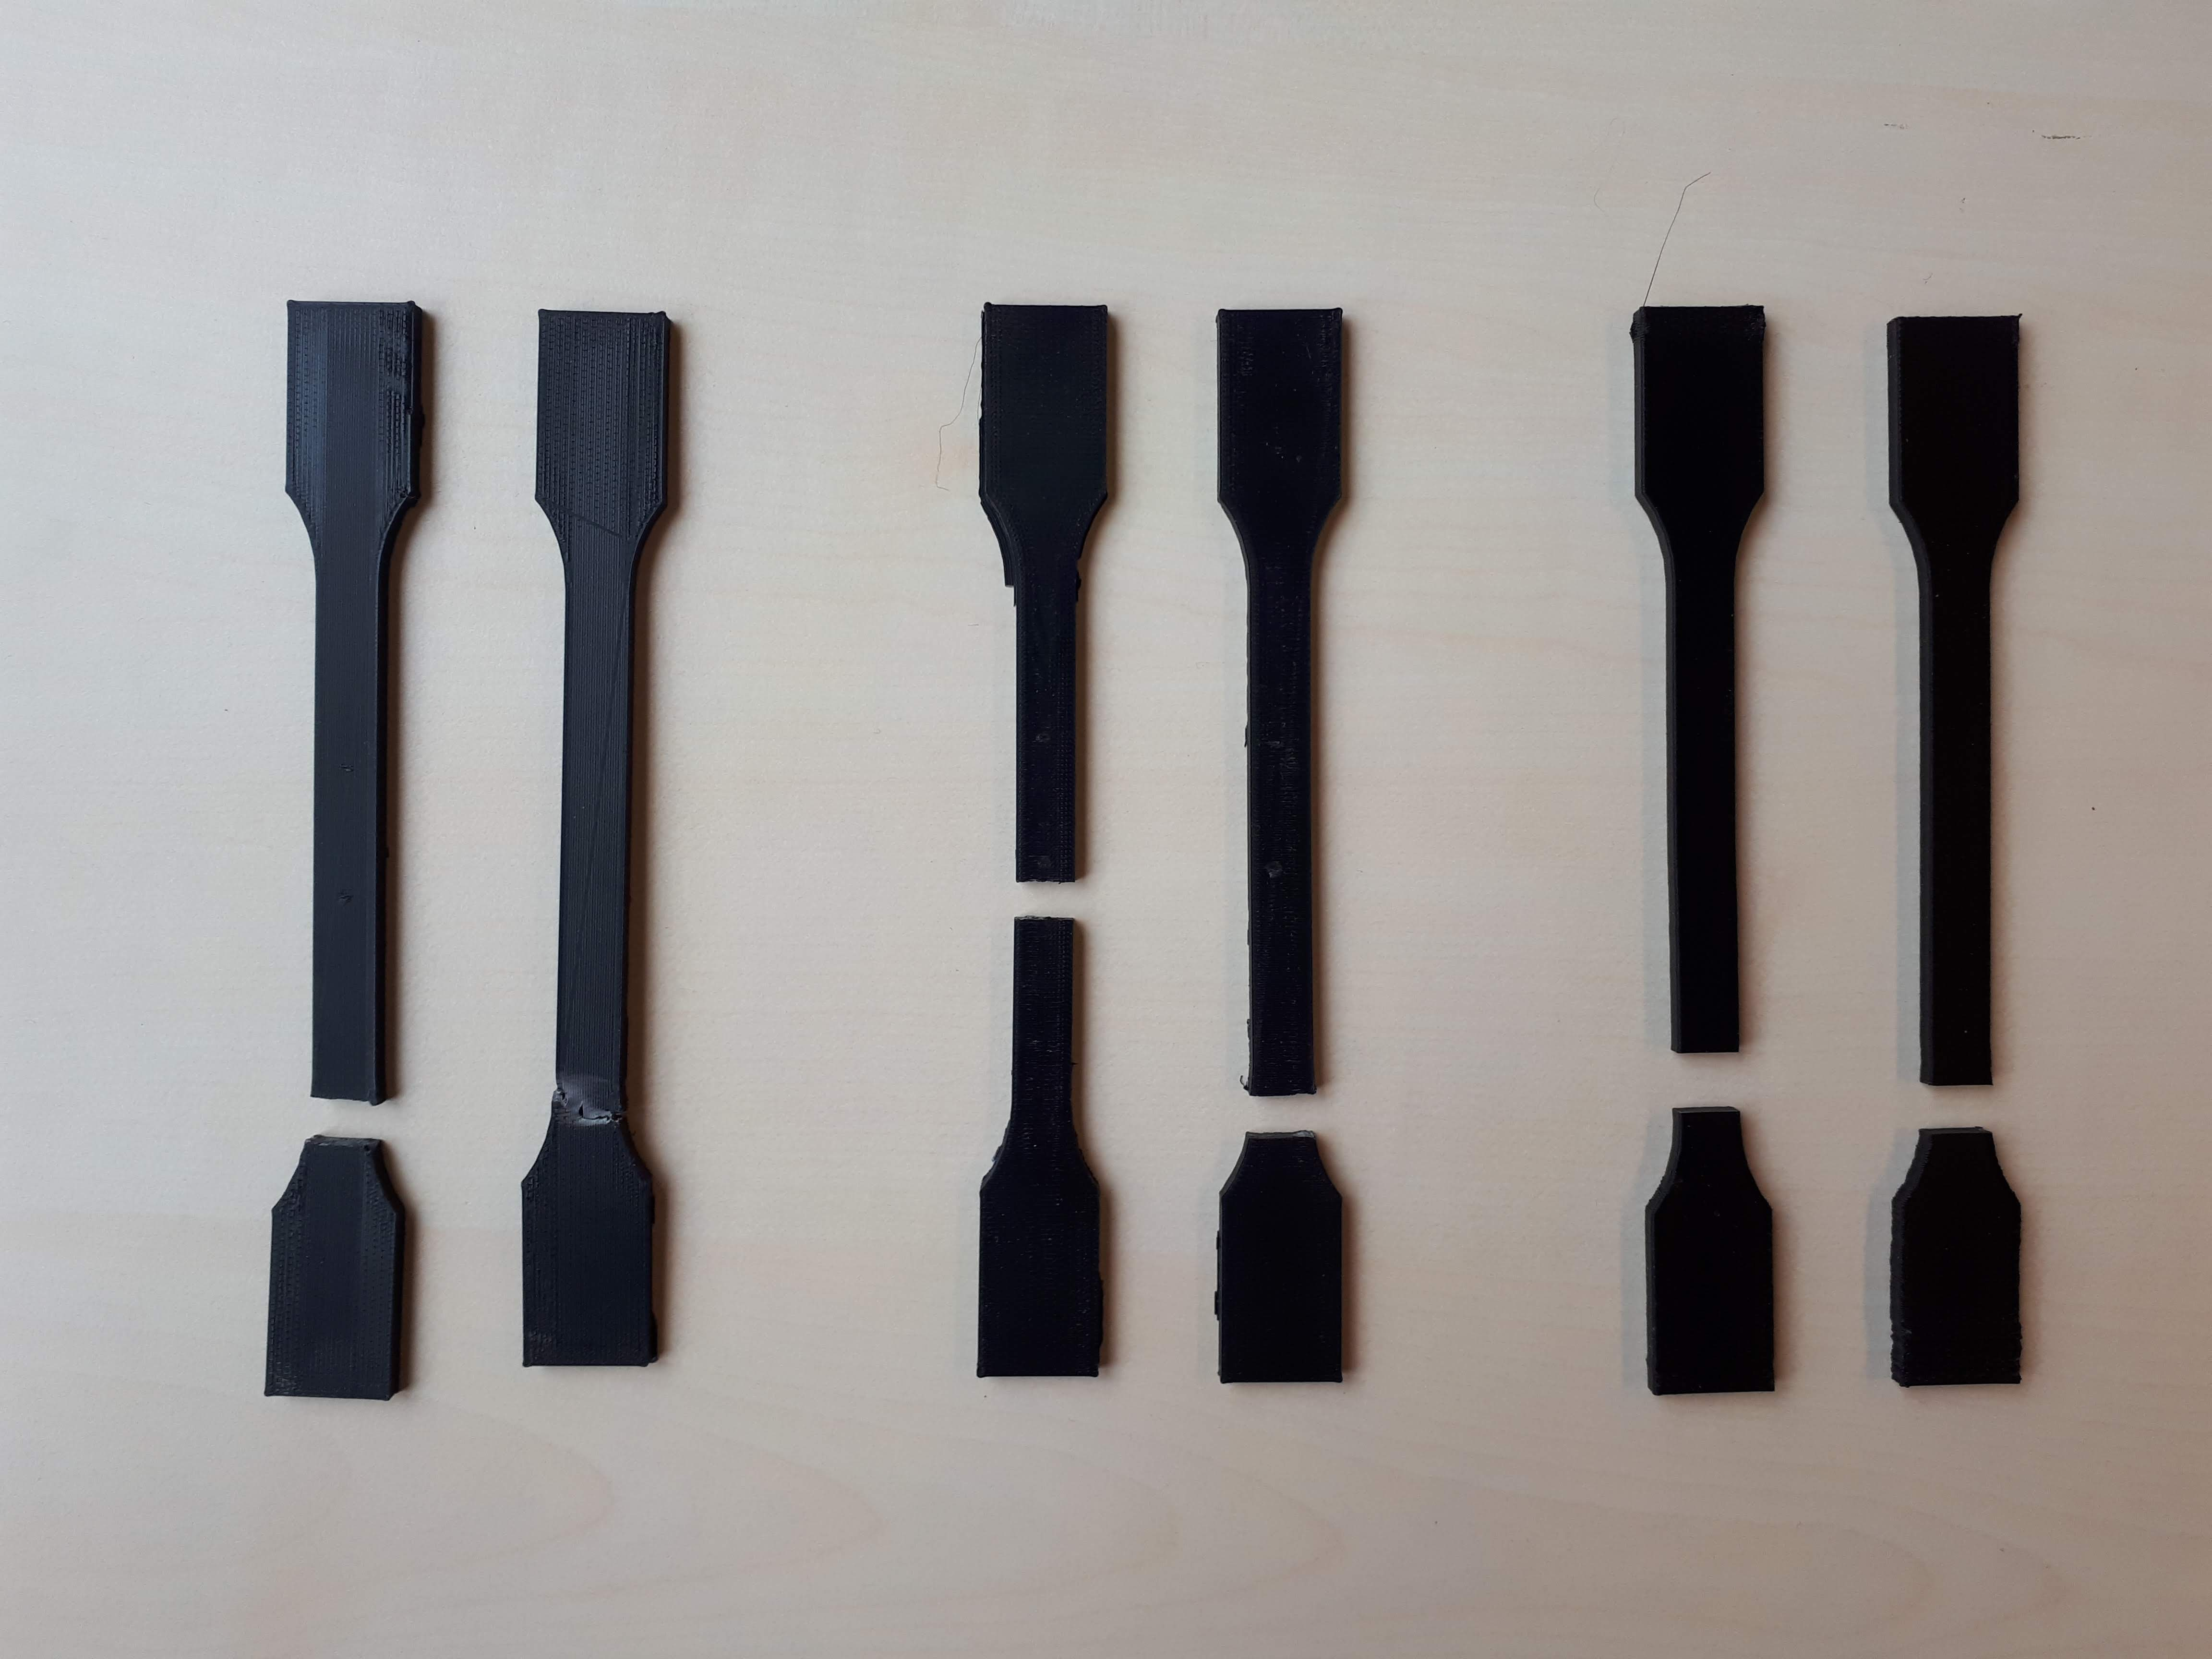
\includegraphics[width=0.40\textwidth]{chapter_5_Experimentaltesting/figures/imageISO.jpg}
    \caption{Tested sepcimen, left: YX[0], middle: XY[0] right ZY[0]}
    \label{fig:ISO527specimen}
\end{figure}
The results of these specimen show significant brittle failure (especially in the XY[0] and ZY[0] direction). Most of the specimen failed in the region near the fillet of the specimen. The ZY[0] specimen all failed at approximately the same point, at the beginning of the fillet. 

\subsection{ASTM D 3039}
\subsubsection{No wall layers }
In figure \ref{fig:ASTM3039results} and table \label{tab:ASTM3039results} the results are presented of the ASTM 3039 samples with no wall layers.
\begin{figure}[H]
    \centering
    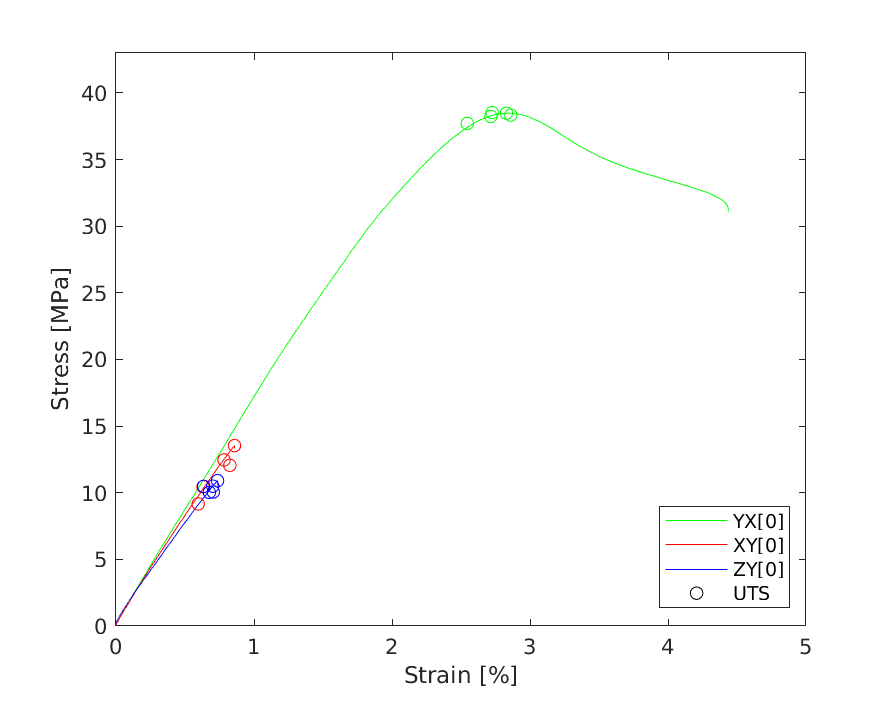
\includegraphics[width=0.80\textwidth]{chapter_5_Experimentaltesting/figures/ASTMnoTensiletests.png}
    \caption{Stress strain curves of the ASTM 3039 samples with no wall layers}
    \label{fig:ASTM3039results}
\end{figure}
In figure \ref{tab:ISO527results} the tested specimen of the ISO 527 samples are shown. 

\begin{table}
\centering
\caption{Properties of the ASTM D 3039 tests in the 3 principle directions}
          \label{tab:ASTM3039results}
\begin{tabular}{ p{1.5cm}p{1cm}p{1cm}p{1cm}p{1cm}p{1cm}p{1cm}  }
\hline
direction & $E$ avg. [MPa] & $E$ std. dev. & $\sigma_y$avg. [MPa] & $\sigma_y$ std. dev. & $\epsilon_y$ avg. [\%] & $\epsilon_y$   std. dev. \\
 \hline
1 (YX[0]) & 1811 & 62 & 39.1 & 0.29 & 2.84 & 0.11 \\
2 (XY[0]) & 1616 & 85 & 11.4 & 2.21 & 0.73 & 0.14 \\
3 (ZY[0]) & 1606 & 64 & 9.9 & 0.65 & 0.61 & 0.04\\
 \hline
\end{tabular}
\end{table}

In figure \ref{fig:ASTM3039WLresults} the tested specimen of the ASTM 3039 samples with no wall layers are shown.
\begin{figure}[H]
    \centering
    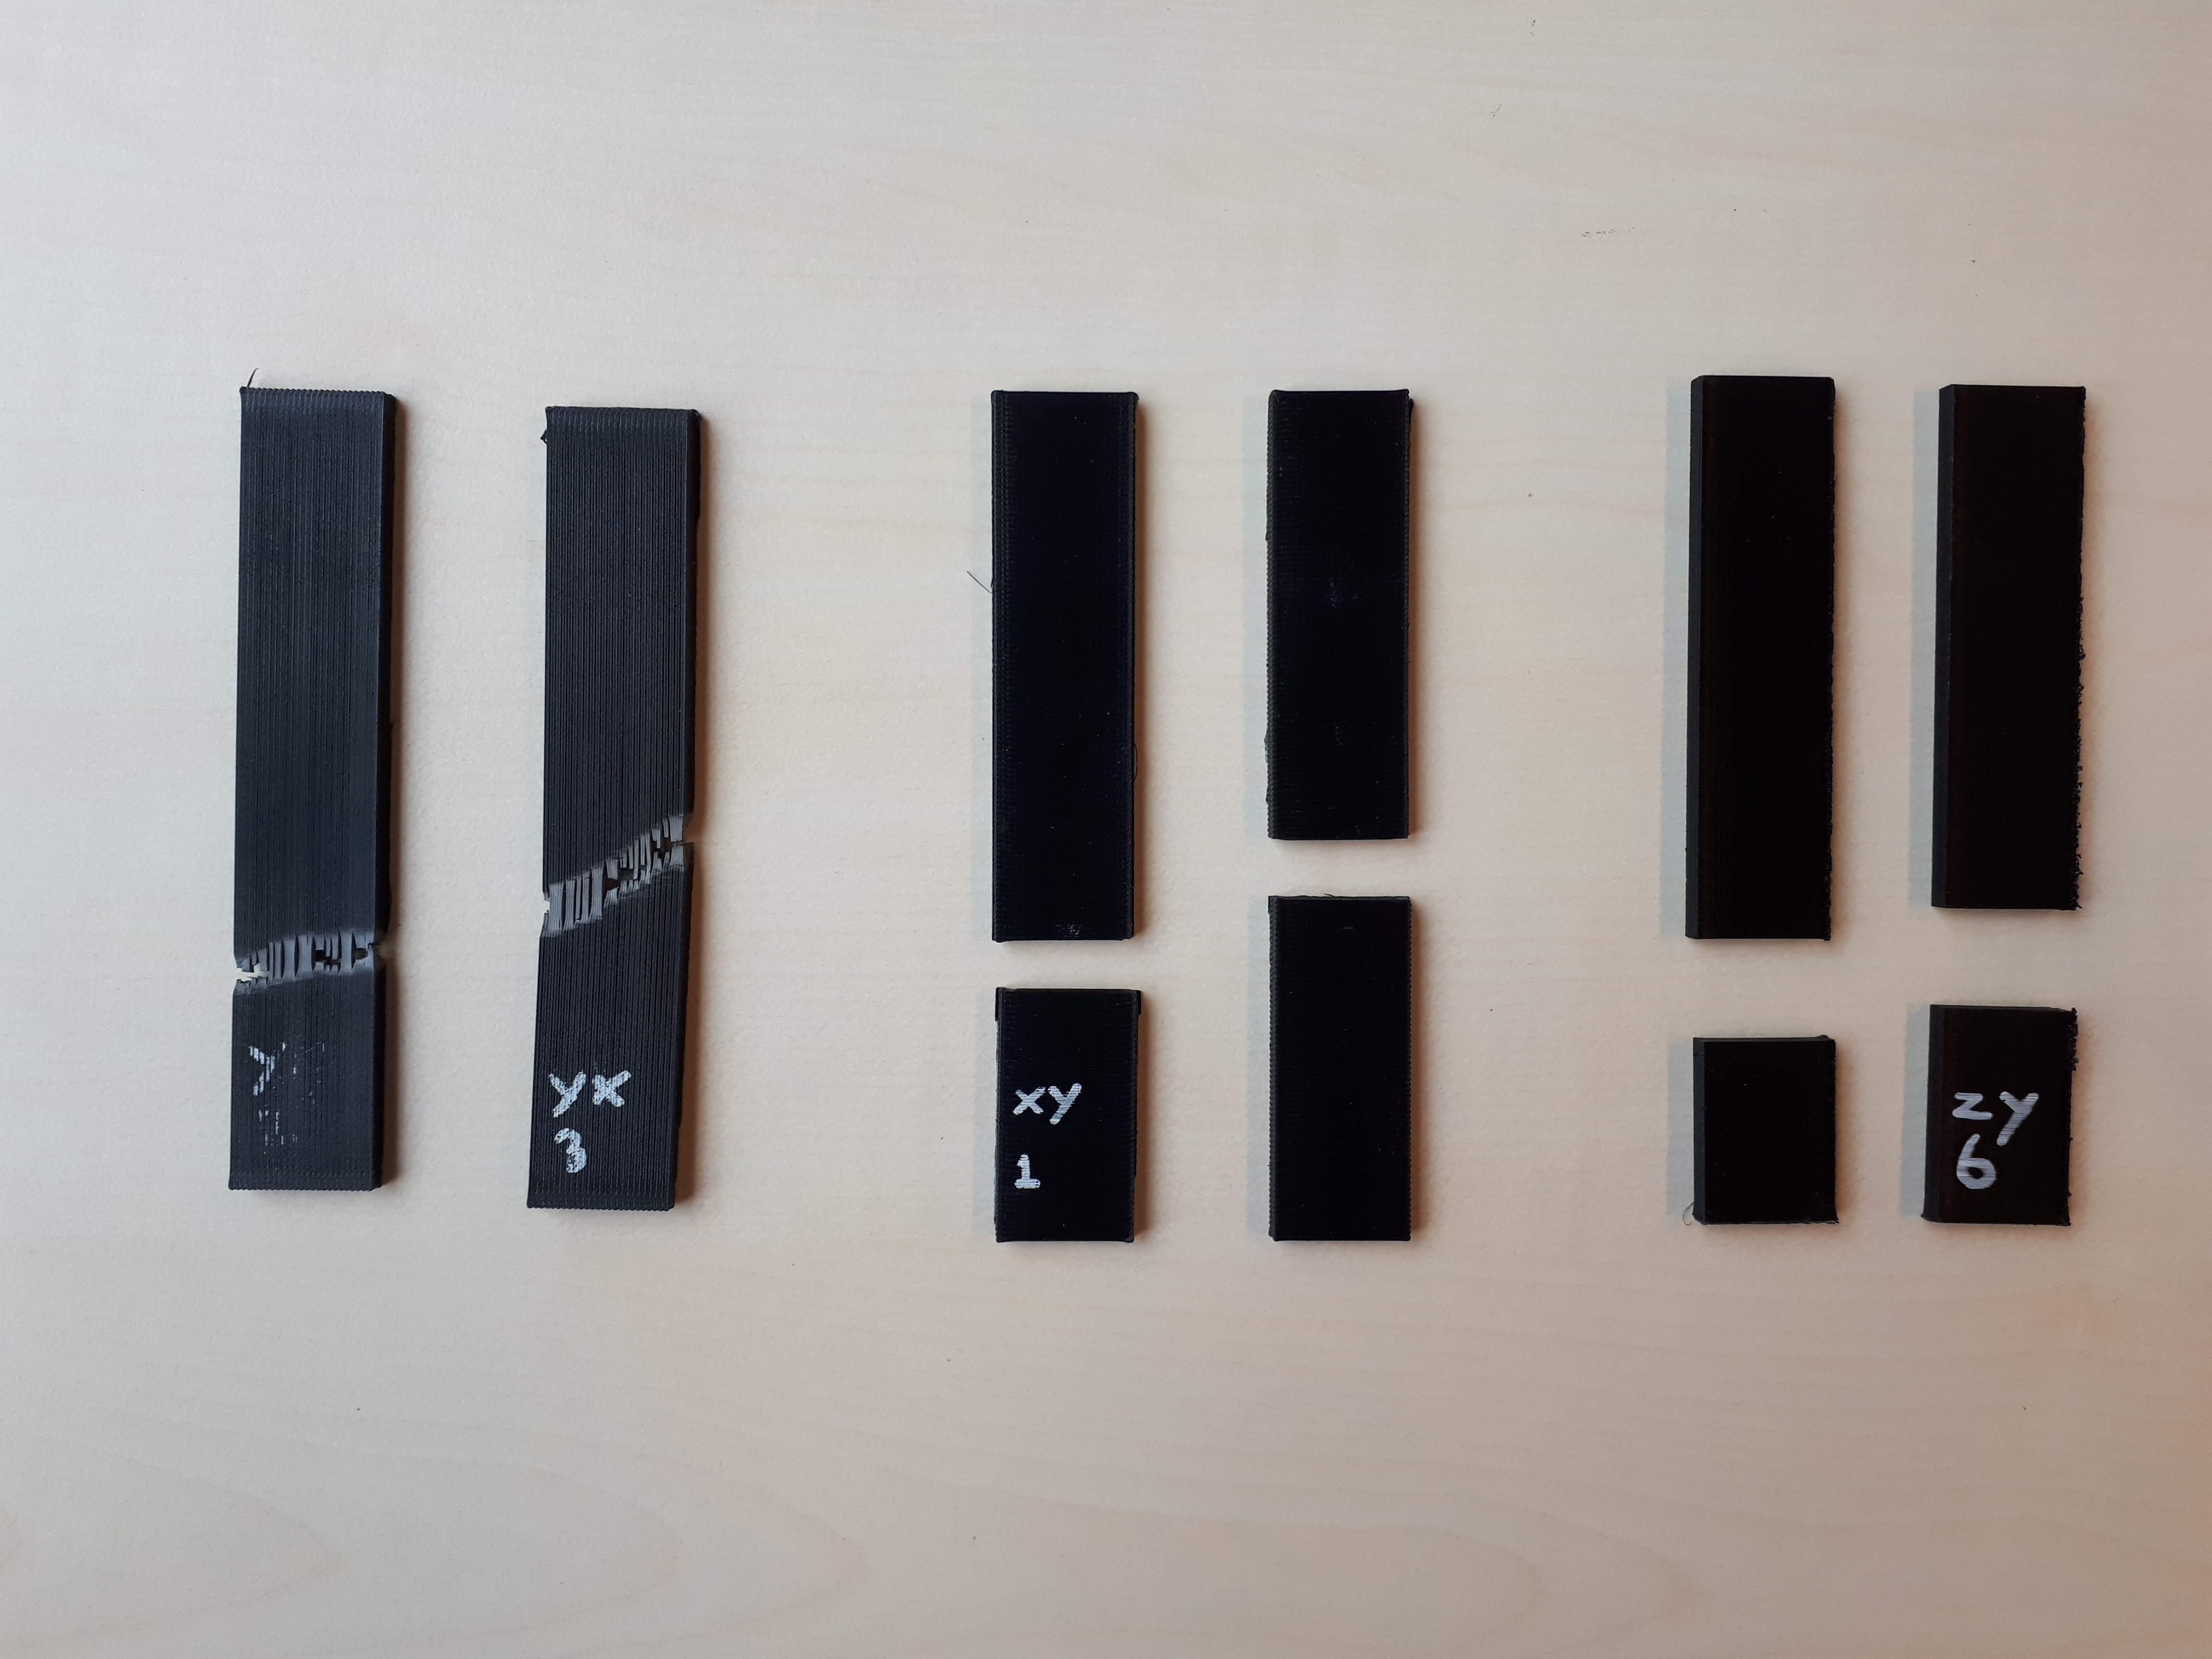
\includegraphics[width=0.40\textwidth]{chapter_5_Experimentaltesting/figures/ImageASTM.jpg}
    \caption{ASTM Tested sepcimen, left: YX[0], middle: XY[0] right ZY[0]}
    \label{fig:ASTM3039specimen}
\end{figure}
The YX[0] specimen showed much more ductile behaviour in comparison with the ISO 527 samples. However, the XY[0] and ZY[0] still showed significant brittle behaviour. The ZY[0] specimen failed again in the region near the clamps.

\subsubsection{Additional} 
In figure \ref{fig:ASTM3039WLresults} and table \label{tab:additionalresults} different results are presented of ASTM 3039 XY samples. A set without wall layers, a set with wall layers and a set with XY[45] samples.
\begin{figure}[H]
    \centering
    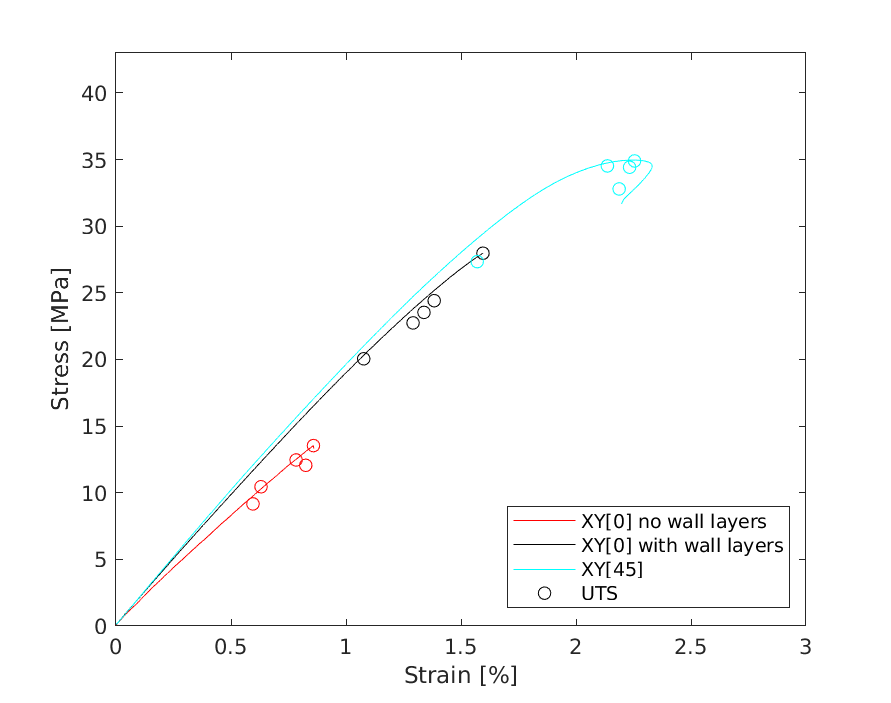
\includegraphics[width=0.80\textwidth]{chapter_5_Experimentaltesting/figures/ASTMWLTensiletests.png}
    \caption{Stress strain curves of the ASTM 3039 XY samples, without wall layers, XY[0] with wall layers and XY[45] with wall layers.}
    \label{fig:ASTM3039WLresults}
\end{figure}

\begin{table}
\caption{Properties of the additional ASTM D 3039 tests in the 3 principle directions}
\begin{tabular}{ p{2.5cm}p{1cm}p{1cm}p{1cm}p{1cm}p{1cm}p{1cm}  }
 \hline
direction & $E$ avg. [MPa] & $E$ std. dev. & $\sigma_y$avg. [MPa] & $\sigma_y$ std. dev. & $\epsilon_y$ avg. [\%] & $\epsilon_y$   std. dev. \\
 \hline
XY[45] & 1945 & 72 & 32.8 & 2.83 & 2.07 & 0.26 \\
XY[0] (No WL) & 1616 & 85 & 11.4 & 2.21 & 0.73 & 0.14 \\
XY[0] (WL)& 1879 & 70.5 & 22.9 & 3.36 & 1.3 & 0.21\\
 \hline
\end{tabular}
     \label{tab:additionalresults}
     \end{table}


In figure \ref{fig:ASTM3039addspecimen} the tested specimen of the ASTM 3039 samples with no wall layers are shown.
\begin{figure}[H]
    \centering
    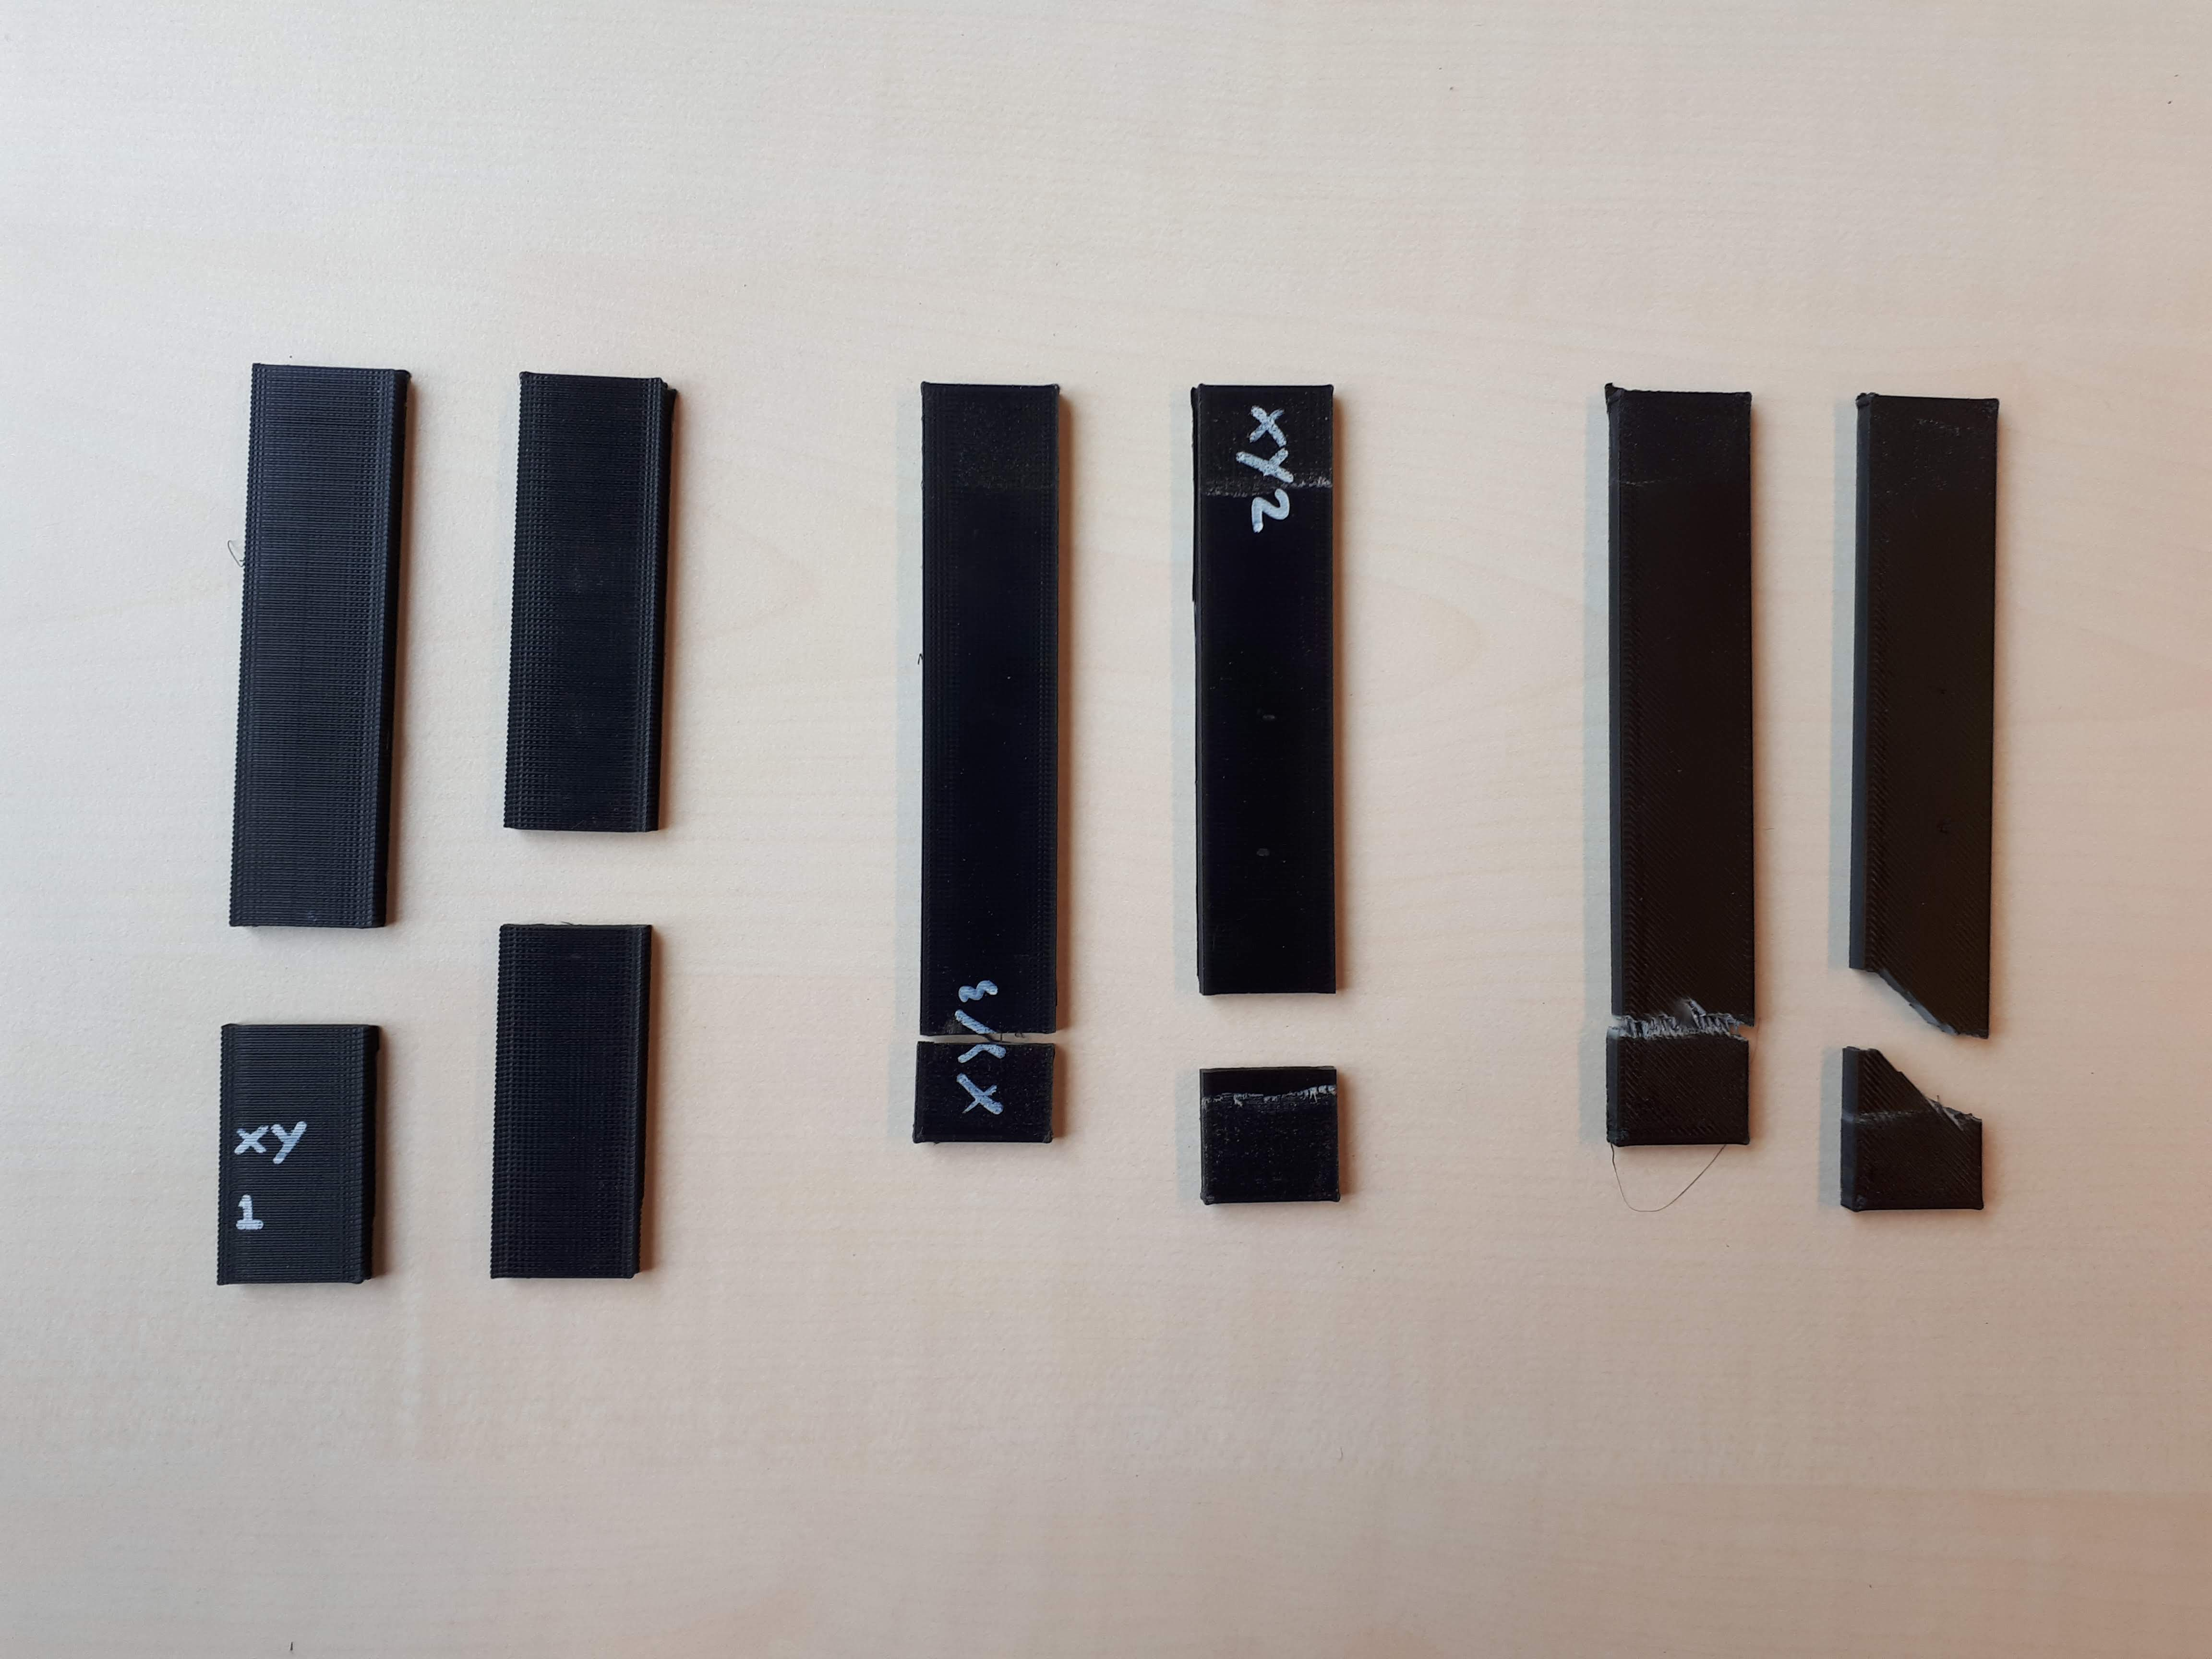
\includegraphics[width=0.40\textwidth]{chapter_5_Experimentaltesting/figures/imageASTMadd.jpg}
    \caption{ASTM additional tested specimen, left: XY[0] (no WL), middle: XY[0] (WL) right XY[45]}
    \label{fig:ASTM3039addspecimen}
\end{figure}
The XY[0] sample with wall layers showed less brittle behaviour, and had a significant increase in yield strength. The XY[45] sample showed  more ductile behaviour, even reaching the softening region.


\subsection{Ultimaker ABS Filament}
In figure \ref{fig:filamentresults} and table \ref{tab:additionalresults} the results of the Ultimaker ABS filament are presented.
\begin{figure}[H]
    \centering
    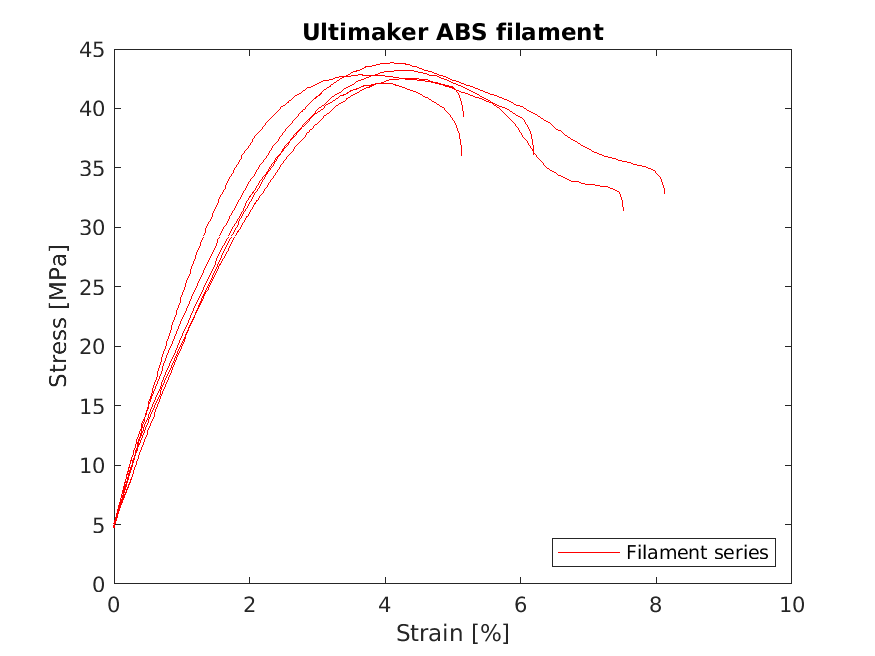
\includegraphics[width=0.80\textwidth]{chapter_5_Experimentaltesting/figures/filamentdata.png}
    \caption{Stress strain curves Ultimaker ABS filament}
    \label{fig:filamentresults}
\end{figure}
Be aware that the stress strain curve is moved 0.225\% to the right to determine the average representative properties. The sample was pre-loaded with 5 MPa to straighten the filament out, this corresponded to approximately 0.225\% strain. This only affects the effective strain at yield and break.

\todo{Check if I found the correct reference used in Table 5.4.}

\begin{table}
\caption{Properties of the tested filament}
\begin{tabular}{ p{1.5cm}p{1cm}p{1cm}p{1cm}p{1cm}p{1cm}p{1cm}p{1cm}p{1cm}  }
 \hline
direction & $E$ avg. [MPa] & $E$ std. dev. & $\sigma_y$avg. [MPa] & $\sigma_y$ std. dev. & $\epsilon_y$ avg. [\%] & $\epsilon_y$   std. dev. & $\epsilon_b$ avg. [\%] & $\epsilon_b$   std. dev \\
 \hline
Exp. filament & 2019 & 81.3 & 42.8 & 0.57 & 4.27 & 0.26 & 6.52 & 1.44\\
Injection molded \cite{Ultimaker2018TechnicalABS} & 2030 & - & 43.6 & - & 4.8 & - & 34 & -\\
 \hline
\end{tabular}
     \label{tab:additionalresults}
 \end{table}
% Discuss comparison with UM spec sheet.

In figure \ref{fig:filamentresults} the tested specimen of the ABS filament are shown.
\begin{figure}[H]
    \centering
    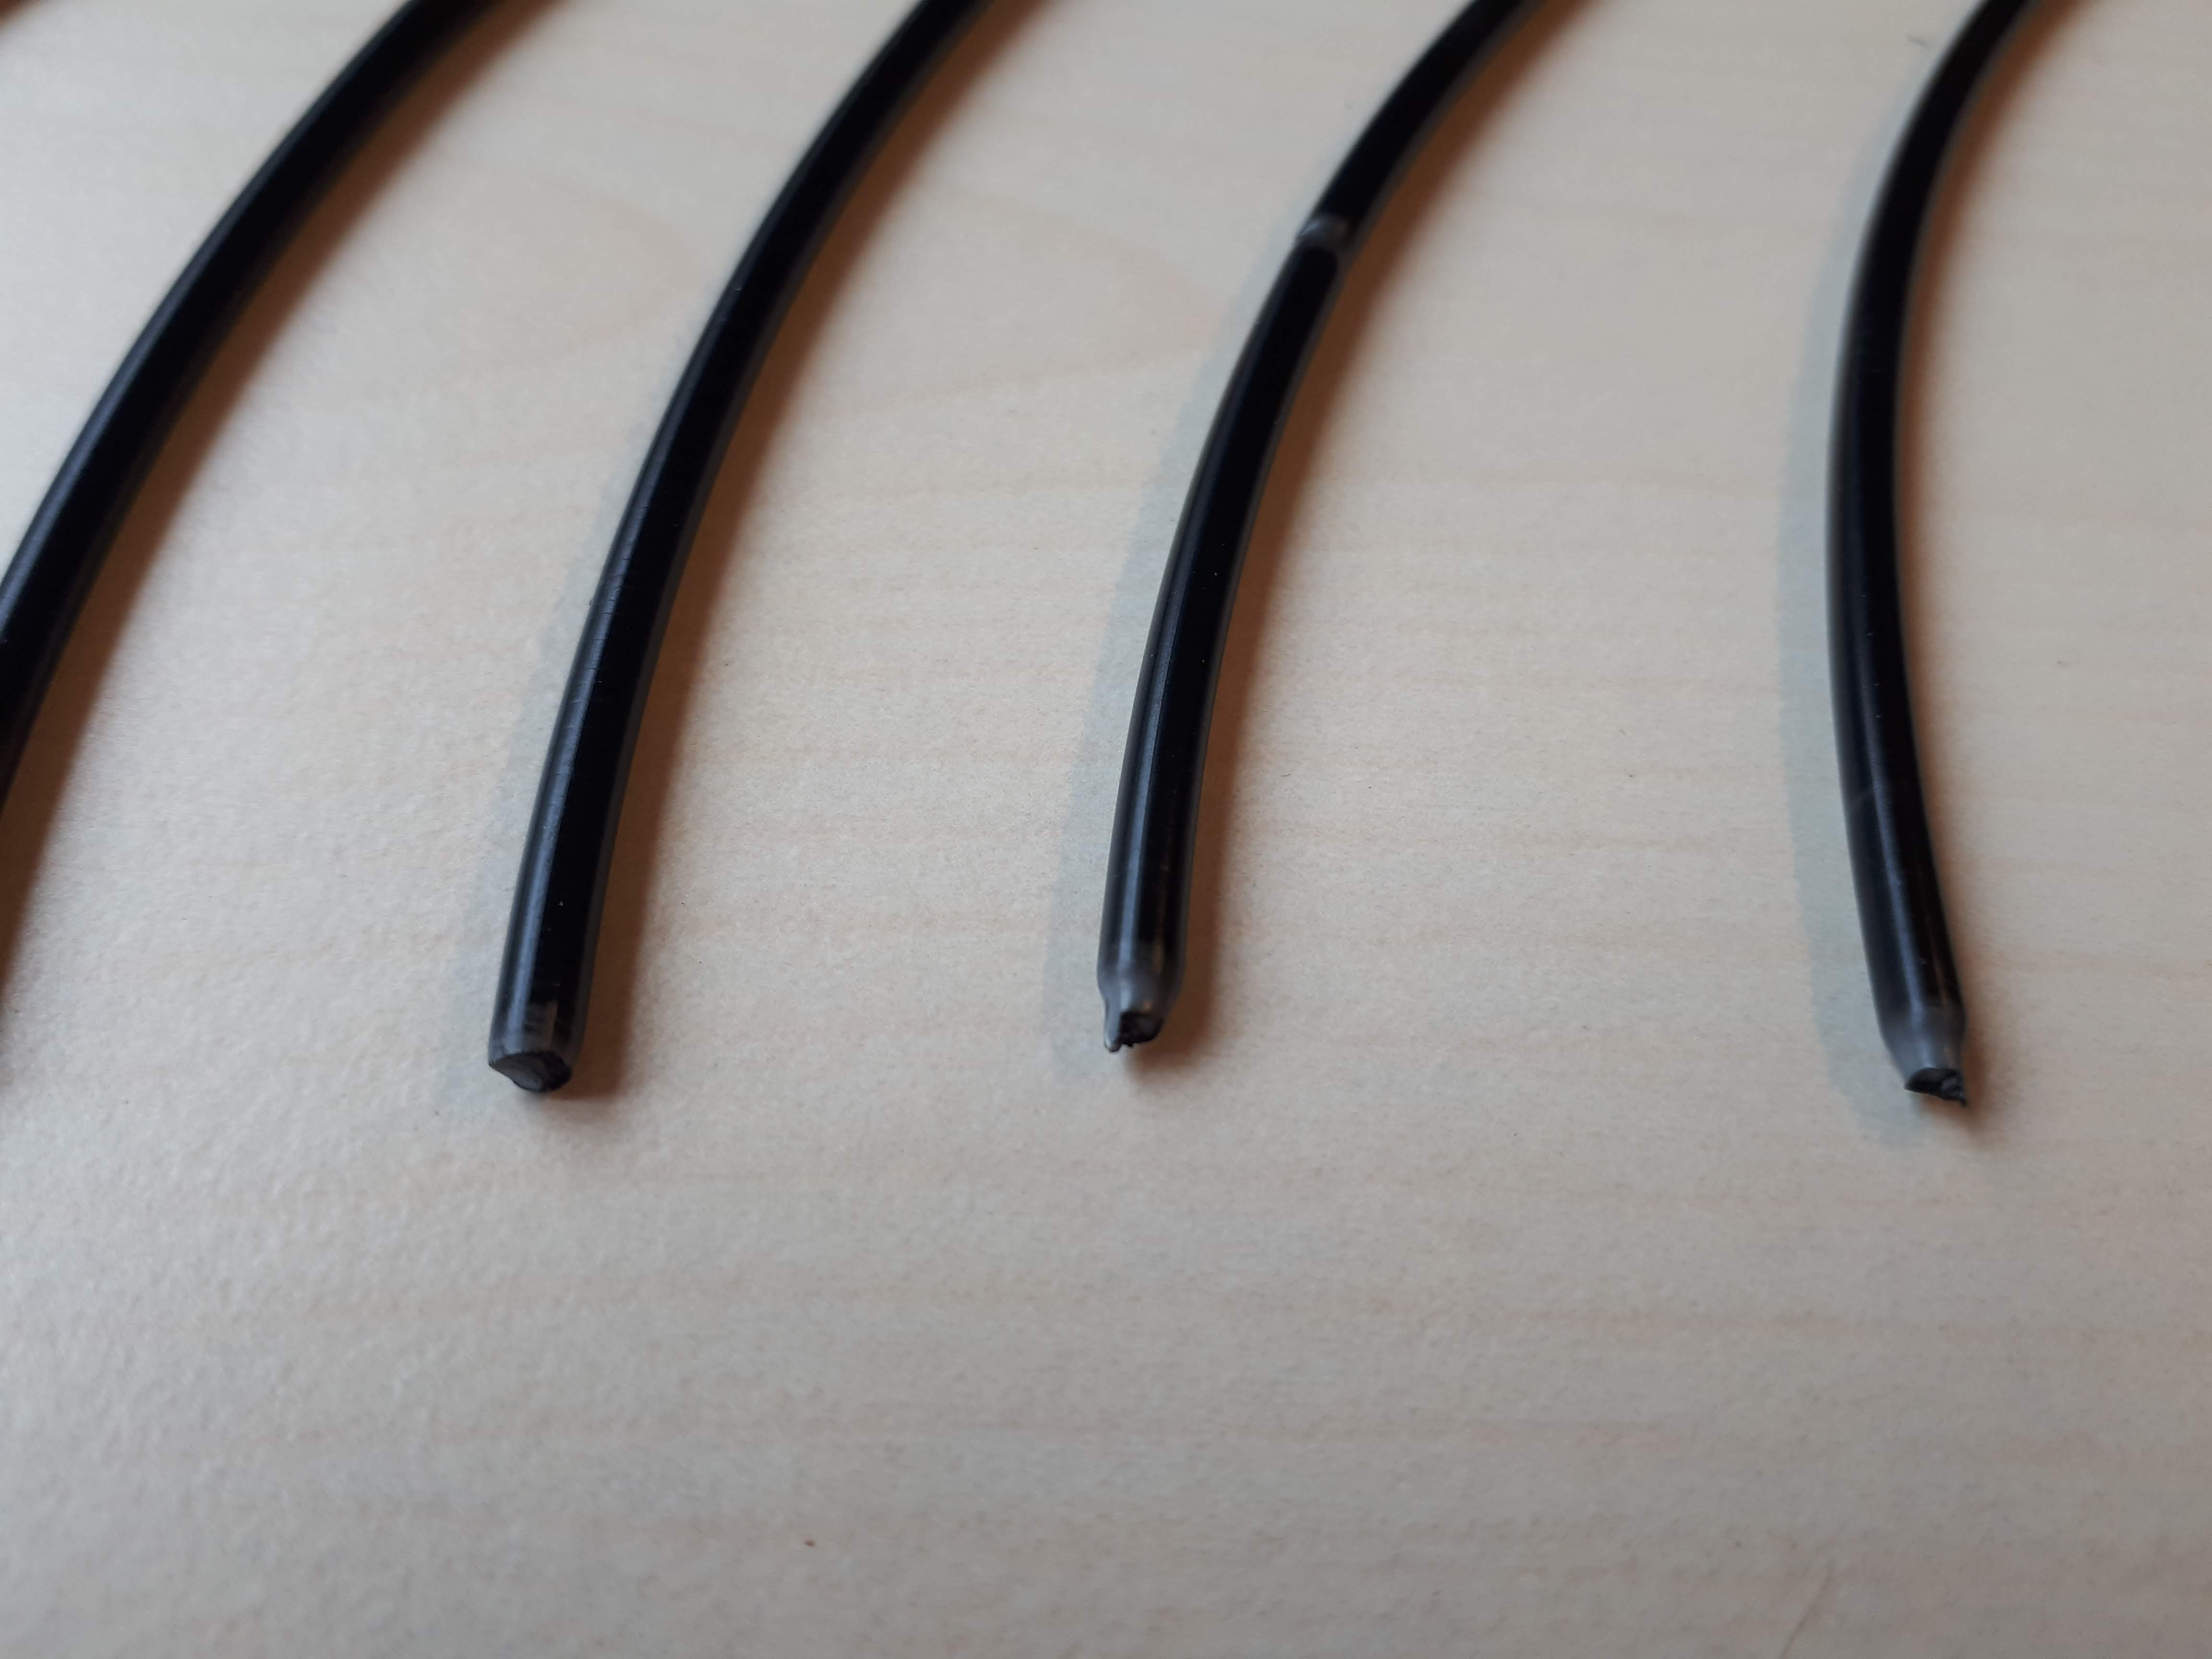
\includegraphics[width=0.40\textwidth]{chapter_5_Experimentaltesting/figures/Imagefilament.jpg}
    \caption{Tested Ultimaker ABS filament}
    \label{fig:filamentspecimen}
\end{figure}
The set of tested filament showed a similar behaviour, but had significant difference in break point. Nonetheless the yield points are quite close to each other. The tested specimen show some whitening, which would indicate plastic deformation.  

\section{Discussion}
%why?
The conducted experimental tensile tests of FFF produced specimen were produced to create a benchmark and to validate the FEM model that was created to predict the behaviour of FFF produced part. The tests of the ABS filament is used to create hardening curves that are imported in the FEM model. Overall, these tests also verify the results in the literature and give significant insight on the behviour of FFF produced parts. 
%external affectors, test standards
During these test it is observed that the production technique, test method and environment had significant impact on the response of the stress strain curve. As has been analysed in the literature in chapter 2, the production parameters are inherently linked to the properties of FFF produced parts. Therefore, a standard set of production parameters, which have proven to generate decent results, and that were close to the conducted experiments in literature, are chosen. This thesis will not investigate the effect of different process parameters empirically. The test method, where the most influential  parameters include the geometry of the specimen and the strain rate, proved to significantly alter the response of the test. The ISO 527 specimen (dogbone shaped) exhibited major complication during testing. Failure is predominantly brittle and initiated at the beginning of the fillets. This is probably due to stress concentrations and crack initiation points. 

Be aware that the geometry and printing strategy also affects the temperature history of a certain road interface. For example, the time a toolhead passes an interface of a adjacent road is much shorter in the xy plane than the z direction, since the printer first finishes a layer before moving in the z direction to a new layer. Therefore, considering the parameters in table \ref{tab:parameters}, the toolhead in the xy plane for the XY[0] ASTM D 3039 test samples will reach the adjacent road 10 times faster than the inter layer interfaces for the respective ZX[0] sample (1 second versus 10 seconds). Accoding to the healing theory, this would lead to a better healed interface for the XY[0] samples perpendicular to the loading direction, compared to the ZX[0] samples, assuming they are not fully headed. The results in figure \ref{fig:ASTM3039results} support this due to the lower UTS measured for the ZX[0] samples. However, we do not yet know if this is affected by the healing or by the difference in mesostructure. This will further be investigated in chapter 7. 
%stress concentrations and crack initiation points
Stress concentration occur when a load is applied along a body with a geometrically altering cross section \cite{TronvollTheApproach}. The "dogbones" are designed to ensure failure in the mid region of the specimen and to compensate for the stress of the grips. However, for an isotropic material, which applies for FFF parts, stress might not be transferred homogeneously, creating stress concentrations. Additionally, crack initiation points at the surface are produced during the production process, this is due to the sintering of the roads. Finally, the internal pores also act as crack initiation points. To limit the effect of the surface roughness and stress concentration, the ASTM 3039 standard was chosen to have a even cross section along the specimen. The results show that the ASTM 3039 samples provide a significant better response in the 1 direction, which implies that there is less stress concentration leading to brittle failure. Adding wall layers in the ASTM 3039 samples also significantly increases the response (factor 2) but still does not reach a softening region. The ASTM 3039 samples in 1 direction perform better than the ISO sample, but under-performs in the 2 direction. This might be caused by the stress induced by the grips, which is supported by the observation of failure at the start of the gripping area in the ASTM 3039  XY[0] and ZY[0] directions. The ZY[0] ISO 527 samples exhibit a significantly better (increase of 5MPa) compared to the ASTM 3039 samples, this can be attributed to the same phenomenon as is described for the XY[0] direction.
%45 degrees.
The XY[45] sample shows significantly higher ductile response in comparison with the YX[0]. Since the load is not fully perpendicular on the interface of the roads, the road is also loaded in tension, which explains the better response.
%filament
The results from the filament test show a response that is specific to thermoplastics, showing a quasi-linear elastic region followed by a yield point and softening, and ends in a perfect plastic plateau. This curve is characterized as a C curve in different standards \cite{Afd2016NEN-EN-ISO527-2},\cite{Fahrenholz2018TheZwick/Roell}. The filament inhibits less plasticity than would be expected \cite{Rodriguez2001MechanicalInvestigation}. Since this filament has been stored in an unconditioned room, there is a large possibility of moisture uptake, which decreases the ductile properties of the filament \cite{Turner2014AModeling}. This can explain the difference between the observed strain at break and the strain at break from the technical data sheet \cite{Ultimaker2018TechnicalABS}. \todo{Again, replaced TechnicalUM citation}
%strain rate
The filament has been tested on a relatively high strain rate to determine the stress strain curve, the technical datasheet provided by Ultimaker prescribed a strain rate of 50mm/min. Higher strain rates lead in general to a harder (higher UTS and lower elongation at break) response, since they limit the visco-elastic behaviour of the plastic. Following this method the results for the Youngs modulus and yield point were close to the provided technical data sheet, for $E, \sigma_y, \epsilon_y$ respectively 0.5\%, 1.83\% and 11.04\% lower. The strain at break is much higher for the injection molded data, this might be due to the sample form of the injection molded sample and additionally due to the absorbed moisture by the ABS filament.  

When importing these hardening curves in a FEM model one should take into account the limited visco-elastic behaviour. 

\section{Conclusion}
Different methods were used to determine the properties of FFF parts in different directions. The results between methods differ, but can be attributed to the geometry and method of the test standard. No optimal method was found for testing the three principle directions. With the generated results, it can be concluded that there is significant an-istropy  between directions. The 1 direction shows a ductile behaviour while the 2 and 3 directions a very brittle behaviour. Since it was concluded that the RVE shows large porosity, and the strength of the FFF is largely governed by the healing  between roads, the probable mechanism of failure is crack initiation at stress concentrations were roads have sub-optimal healing. These phenomena are in line with the theory on polymer physics as is discussed in chapter 2. The validation and additional knowledge on the behvaiour of FFF products is important in choosing the appropriate constituative relations in the FEM model.  
The RVE model will generate data that would representative of the bulk material with fully healed roads. This data could help identifying the best representative response from the different testing standards.
The hardening curves extracted from the filament tests are close to the data mentioned by the specification sheet. Therefore, these can be useful as input curves for the FEM model. However, since filaments in use are relatively old (multiple months) and have not been stored in a controlled environment, these will likely give a more brittle response. 

%input references to different parts